\documentclass[12pt]{article}
\usepackage{times}
\usepackage{plext}
\usepackage{cite}
\usepackage{setspace}
\usepackage{float}
\usepackage{lineno}
\usepackage{color}
\usepackage[dvipdfmx]{graphicx}
\usepackage{array, booktabs}
\usepackage[top=25truemm,bottom=25truemm,left=30truemm,right=30truemm]{geometry}
\usepackage{threeparttable}
\usepackage{ulem}
%\usepackage{amsmath}
\renewcommand{\figurename}{Fig.}
\renewcommand{\tablename}{Table}
\begin{document}\setcounter{page}{1}
\renewcommand\citeleft{(}
\renewcommand\citeright{)}

\flushleft{\textbf{\large{2020年底魚類現存量調査結果}}}\\
\flushright{金森由妃・成松庸二・鈴木勇人・森川英祐・時岡 駿・\\三澤 遼・永尾次郎(水産機構資源研)
}\\
\ \\

\flushleft{\textbf{背景と目的}\\}
国連海洋法条約では,批准国は領海内の水産資源を適切に管理することが義務付けられている.水産研究・教育機構では,1995年から東北地方太平洋岸沖において底魚類の資源量調査を実施し,主要底魚類の資源状態を調査している.本報告は,2020年秋季に行った調査結果から主要魚種(スケトウダラ,マダラ,イトヒキダラ,キチジ,ズワイガニ,アカガレイ,サメガレイ,ババガレイ)の現存量,分布および体長組成を推定し,過去の結果と比較することで東北地方太平洋岸沖における主要底魚類の資源状況を的確に把握することを目的とした.
\ \\

\flushleft{\textbf{材料と方法}\\}
2020年10月1日~11月13日に青森県尻屋崎沖(北緯$\textrm{41}^\circ \textrm{14}^\prime$)から茨城県日立沖(北緯$\textrm{36}^\circ \textrm{29}^\prime$)までの海域で調査船若鷹丸(水産研究・教育機構所属,692トン)を用いた着底トロール調査を実施した.等深線を横切る8本の調査ライン(A~Hライン)を設定し,A~Dラインを北部海域,E~Hラインを南部海域とした.各調査ラインにおいて水深100m~1000mの間に調査点を設定し,合計107地点で調査を実施した.採集された全魚種について尾数と重量を測定し,主要魚種については体長あるいは甲幅測定を行った.スケトウダラは0歳魚と1歳魚以上,マダラは0歳魚,1歳魚および2歳魚以上,ズワイガニは雌雄に区別して測定した.得られたデータから面積-密度法を用いて南北海域別に現存量・現存尾数と体長組成を推定し,過去の結果と比較した.なお,採集効率は1と仮定した.

\flushleft{\textbf{結果と考察}\\}
スケトウダラの現存量は0歳魚では南北合計1.7トンで,前年の2,000トンから大きく減少した.1歳以上は11,200トンで,前年の5,100より増加した.1歳以上の体長組成では,20 cm台の中型個体が大きく増加した.
\ \\
\hspace{20pt}マダラの現存量は0歳,1歳および2歳以上でそれぞれ1.7トン,1,000トン,3,100トンとなり,0歳と1歳では前年(0歳は180トン,1歳は2,600トン)から減少し,2011年の震災以降最も低い水準であった.2歳以上の体長組成では,前年とおおむね同様の組成を示しており,震災以前のような若齢魚中心の組成と考えられた.
\ \\
\hspace{20pt}イトヒキダラの現存量は7,000トンで,前年の12,000トンから減少した.分布密度について,2015年以前に確認されていた南部の高密度点はみられなかった.体長組成では,北部に体長35 cm以上の中型~大型個体,南部には同様の中型~大型個体に加えて体長30 cm以下の小型個体が多く確認された.
\ \\
\hspace{20pt}キチジの現存量は9,900トンで,前年とほぼ同水準であった.体長組成は南部・北部ともに20 cm前後にピークがあったが,前年と同様に体長10 cm以下の小型個体の山は不明瞭であった.
\ \\
\hspace{20pt}ズワイガニの現存量は雌で54トン,雄は130トンで,雌雄ともに前年より減少した.甲幅組成では,雌雄ともに南北で甲幅サイズが異なる傾向は見られなかった.
\ \\
\hspace{20pt}アカガレイの現存量は170トンで,前年の250トンから減少した.本種の現存量は2018-2019年ではわずかに増加傾向であったが,震災以降は減少傾向であるため,低水準が続いていると考えられる.体長組成では,北部には30-40 cm以上の大型個体,南部には20-25 cmの中型個体のピークが確認された.
\ \\
\hspace{20pt}サメガレイの現存量は950トンで,前年の580トンから増加していたが,この増加は南部よりも北部で大きかった.体長組成では,南部には15--20 cmの小型個体と30 cm前後の中型個体のピークが確認されたが,北部ではピークが不明瞭であった.
\ \\
\hspace{20pt}ババガレイの現存量は570トンで,前年の1,100トンから減少した.体長組成では,南北で体サイズが類似しており,ピークは不明瞭であった.
\ \\
\ \\
\ \\
\begin{figure}[h]
  \centering
  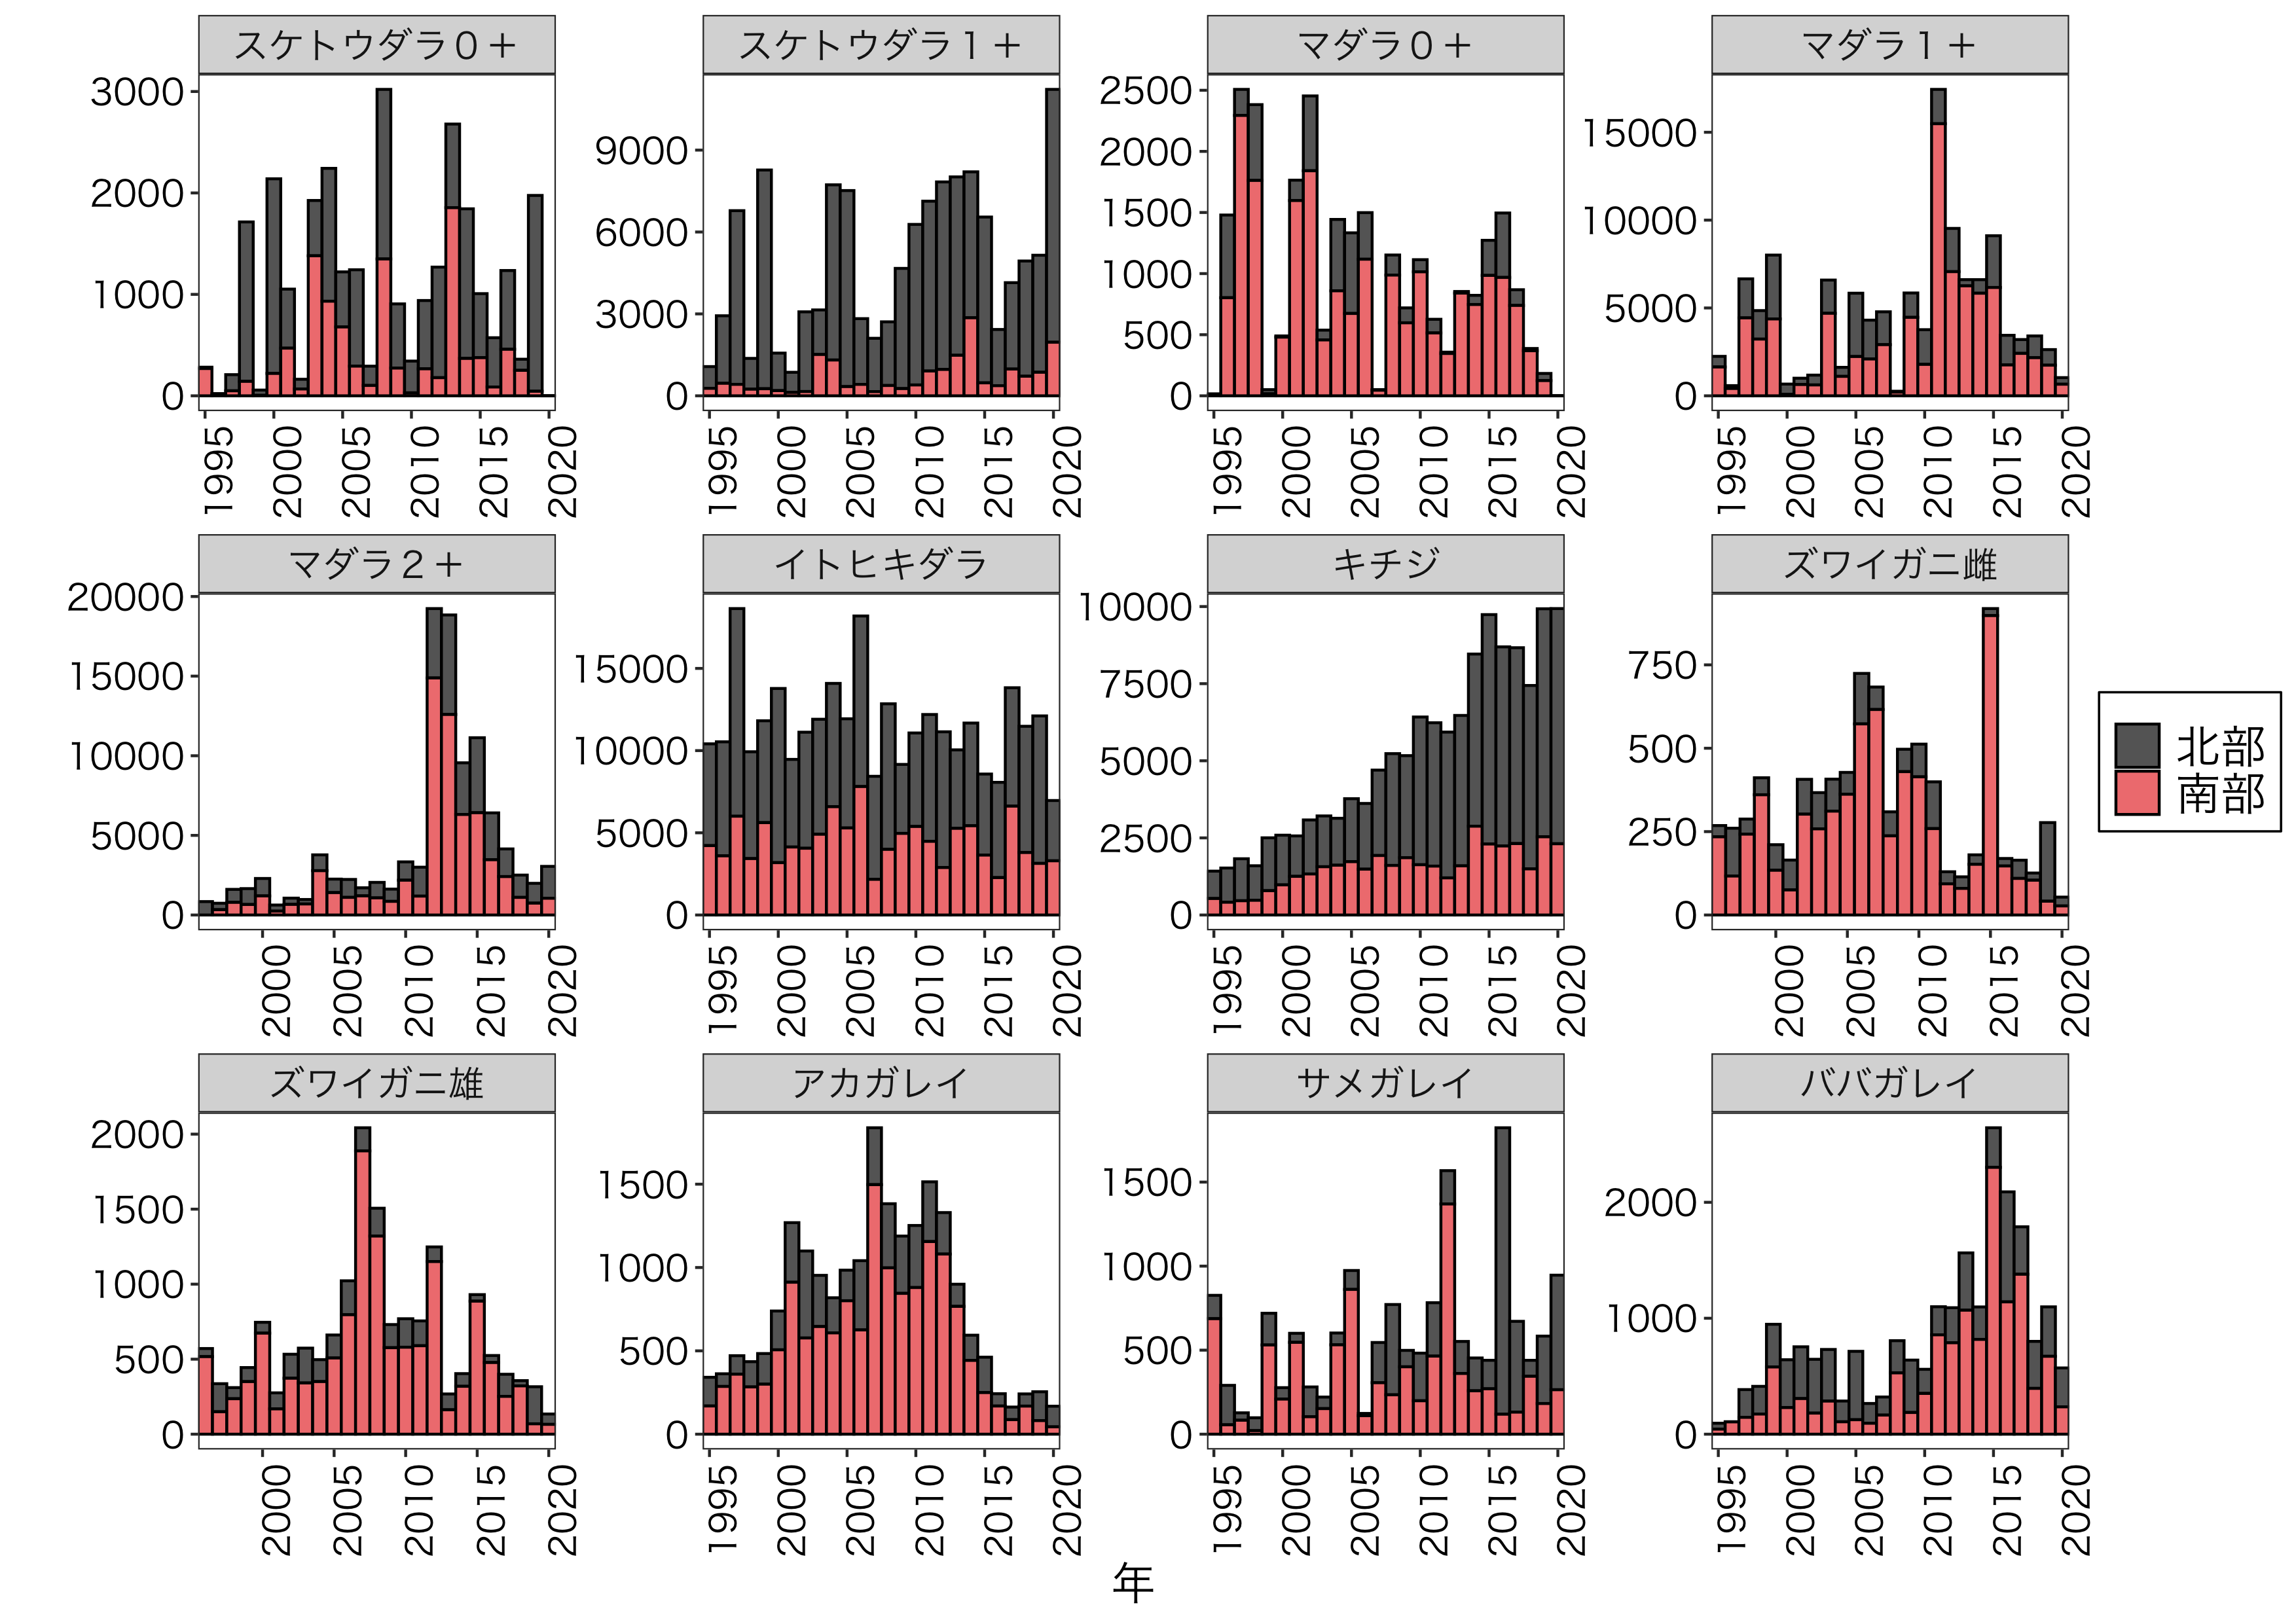
\includegraphics[width = 18cm]{trendabst.png}
  \caption{本発表で報告する主要魚種の現存量の経年変化(単位はトン)}
\end{figure}

\end{document}
